\documentclass[a4paper,12pt]{article}

\usepackage[T2A]{fontenc}
\usepackage[utf8]{inputenc}
\usepackage[russian]{babel}
\usepackage{geometry}
\usepackage{graphicx}
\usepackage{float}
\usepackage{hyperref}
\usepackage{xcolor}
\usepackage{listings}

\geometry{left=25mm,right=15mm,top=20mm,bottom=20mm}
\graphicspath{{./}}
\hypersetup{colorlinks=true,linkcolor=black,urlcolor=blue}
\lstset{
  basicstyle=\ttfamily\small,
  breaklines=true,
  columns=fullflexible,
  frame=single,
  rulecolor=\color{black!25},
  keepspaces=true,
  showstringspaces=false
}

\begin{document}

\begin{titlepage}
\centering
\vspace*{35mm}
{\Large Практическая работа №1\par}
\vspace{6mm}
{\LARGE\bfseries Утилиты настройки сетевых подключений в Linux\par}
\vspace{20mm}
{\large Отчет по выполнению лабораторной работы\par}
\vfill
{\large 2026\par}
\end{titlepage}

\tableofcontents
\newpage

\section{Цель работы}

Цель работы: получить практические навыки настройки сетевых интерфейсов Linux средствами \texttt{ip}, \texttt{nmcli}, \texttt{netplan}, а также настроить bonding-интерфейс и проанализировать счетчики сетевого трафика.

\section{Исходные данные}

В VirtualBox были импортированы две виртуальные машины из OVA:
\begin{itemize}
  \item \textbf{Centos9}: CentOS Stream 9, сетевой адаптер Intel PRO/1000 MT Desktop, MAC \texttt{08:00:27:9a:a4:ef};
  \item \textbf{Debian 12}: Debian 12, сетевой адаптер Intel PRO/1000 MT Desktop, MAC \texttt{08:00:27:c3:04:a5}.
\end{itemize}

В тексте задания указаны CentOS 7 и Debian 11, но фактически предоставленные OVA содержали CentOS Stream 9 и Debian 12. Используемые утилиты и порядок настройки при этом соответствуют заданию.

\section{Часть 1. Скрипт настройки интерфейса}

На Debian был создан пользовательский скрипт \texttt{part1\_net\_menu.sh}. Скрипт работает без изменения постоянных конфигурационных файлов и использует runtime-команды \texttt{ip}, \texttt{resolvectl} и \texttt{dhclient}. Меню содержит пункты:
\begin{itemize}
  \item вывод модели интерфейса, скорости, duplex, состояния link и MAC-адреса;
  \item вывод текущих IPv4-адресов, маршрутов и DNS;
  \item настройка статического сценария \texttt{10.100.0.2/24}, gateway \texttt{10.100.0.1}, DNS \texttt{8.8.8.8};
  \item настройка динамического получения адреса по DHCP;
  \item выход.
\end{itemize}

\lstinputlisting[caption={Скрипт меню для части 1}]{part1_net_menu.sh}

Скрипт был проверен на синтаксис командой \texttt{bash -n}. В информационном режиме интерфейс \texttt{enp0s3} показал драйвер \texttt{e1000}, MAC \texttt{08:00:27:c3:04:a5}, скорость \texttt{1000}, duplex \texttt{full}.

\begin{figure}[H]
\centering
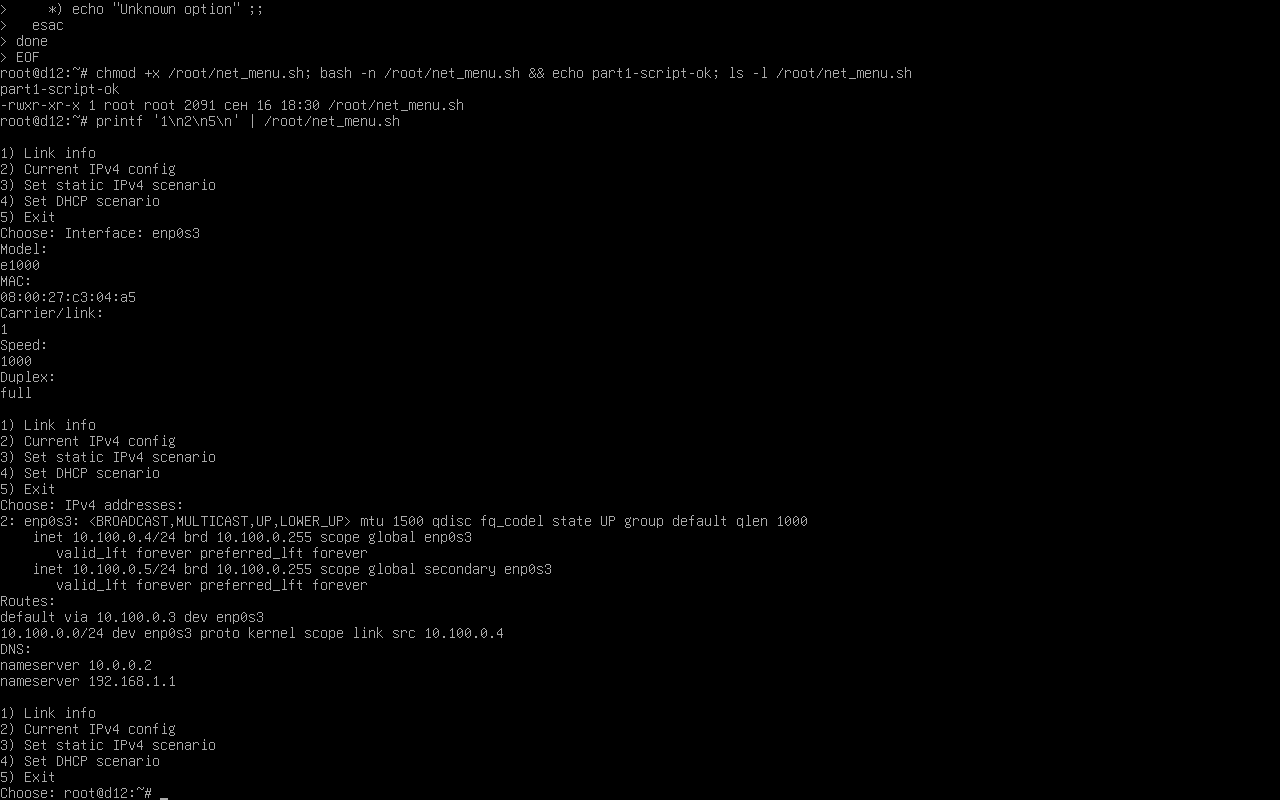
\includegraphics[width=\linewidth]{debian12-part1-output.png}
\caption{Вывод скрипта части 1 на Debian}
\end{figure}

\section{Часть 2. Настройка CentOS через nmcli}

Адаптер CentOS был переведен в режим \texttt{Internal Network} с именем \texttt{seti-lab}. Далее средствами \texttt{nmcli} создан профиль \texttt{lab-static} для реального интерфейса \texttt{enp0s3} и bridge-интерфейс \texttt{br0}.

\lstinputlisting[caption={Runtime-команды nmcli для CentOS}]{part2_centos_runtime.sh}

Результат выполнения:
\begin{itemize}
  \item реальный интерфейс \texttt{enp0s3} получил адрес \texttt{10.100.0.2/24};
  \item bridge-интерфейс \texttt{br0} получил адрес \texttt{10.100.0.3/24};
  \item пинг \texttt{10.100.0.3} и \texttt{10.100.0.2} прошел без потерь;
  \item MAC-адрес \texttt{br0}: \texttt{1a:f3:a6:00:10:6a}.
\end{itemize}

\begin{figure}[H]
\centering
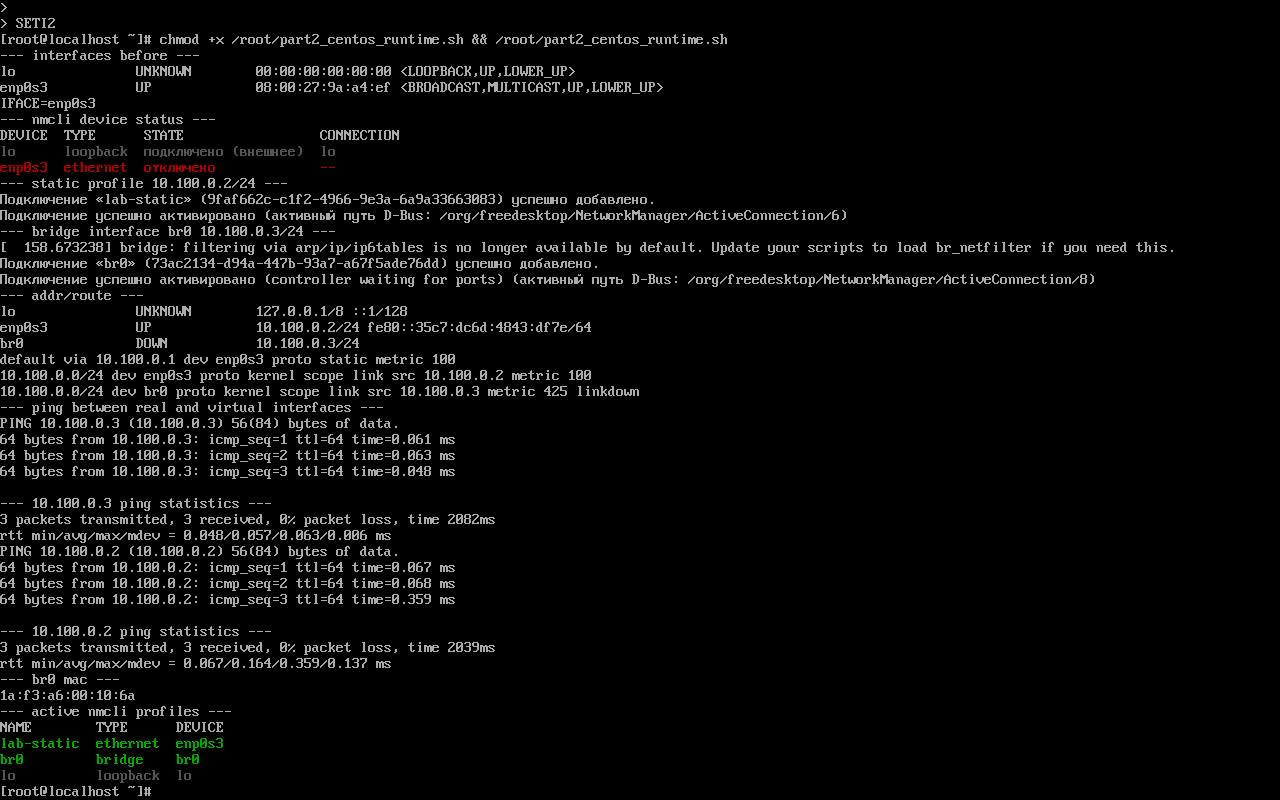
\includegraphics[width=\linewidth]{centos9-part2-output.png}
\caption{CentOS: статический профиль, br0 и проверка связи}
\end{figure}

\section{Часть 3. Debian, netplan и проверка связи}

В Debian был установлен пакет \texttt{netplan.io}. Для интерфейса \texttt{enp0s3} подготовлен файл \texttt{/etc/netplan/99-lab.yaml} со статическими адресами \texttt{10.100.0.4/24} и \texttt{10.100.0.5/24}, маршрутом по умолчанию через \texttt{10.100.0.3} и DNS \texttt{8.8.8.8}.

\lstinputlisting[caption={Файл netplan для Debian}]{part3_debian_netplan_99-lab.yaml}

На предоставленном образе Debian применение через \texttt{netplan apply} вывело ошибку отсутствия службы \texttt{systemd-networkd}. Поэтому для демонстрационной проверки адреса были дополнительно назначены runtime-командами \texttt{ip}; сам YAML-файл сохранен как требуемая постоянная конфигурация.

\lstinputlisting[caption={Runtime-проверка Debian для части 3}]{part3_debian_runtime_check.sh}

Проверка связи:
\begin{itemize}
  \item Debian \texttt{10.100.0.4/5} пингует CentOS \texttt{10.100.0.2}: получено 2 ответа из 3;
  \item Debian \texttt{10.100.0.4/5} пингует CentOS \texttt{10.100.0.3}: получено 3 ответа из 3;
  \item локальные адреса Debian \texttt{10.100.0.4} и \texttt{10.100.0.5} отвечают без потерь;
  \item ARP/neighbor cache Debian содержит удаленные записи \texttt{10.100.0.2} и \texttt{10.100.0.3};
  \item обратная проверка с CentOS показала успешный ping к \texttt{10.100.0.4} и \texttt{10.100.0.5}, а ARP/neighbor cache CentOS содержит записи для этих адресов.
\end{itemize}

Адреса \texttt{10.100.0.4} и \texttt{10.100.0.5} являются локальными адресами Debian, поэтому в ARP-кэше самой Debian они не отображаются как соседние устройства.

\begin{figure}[H]
\centering
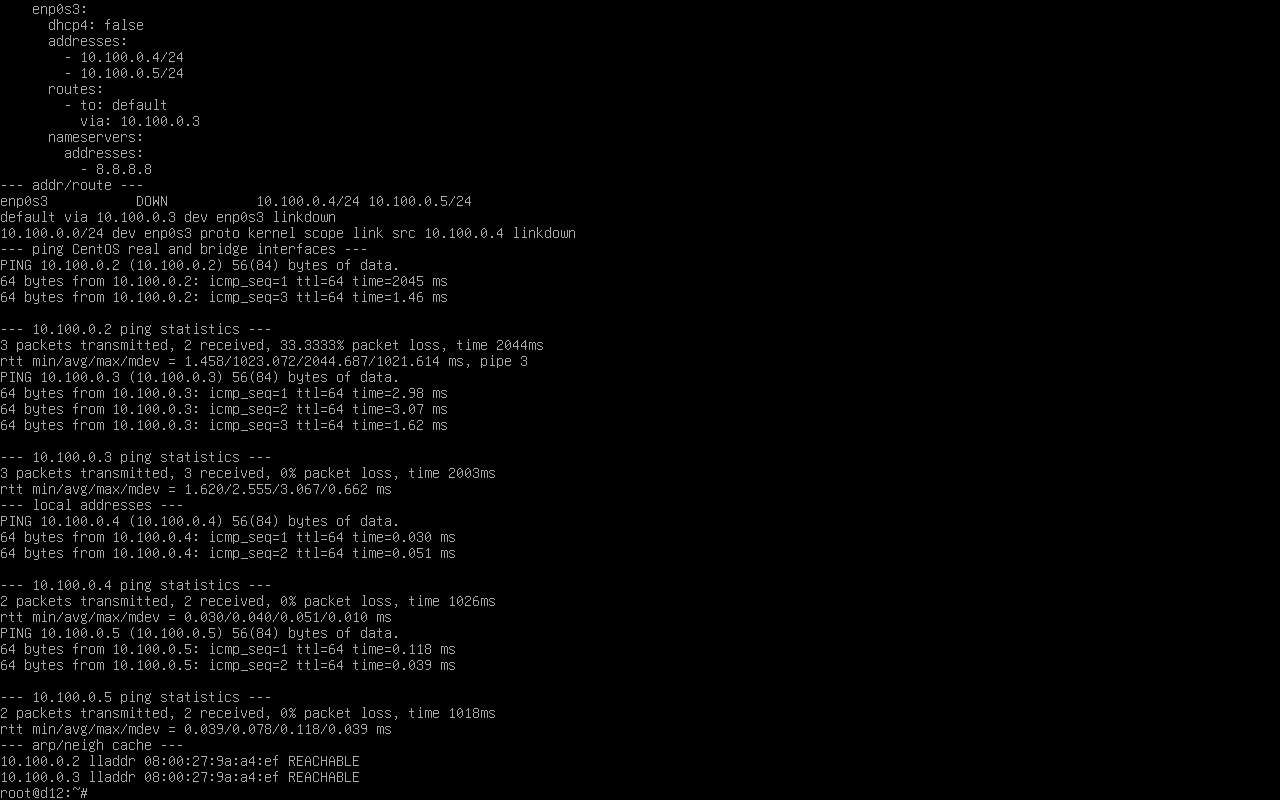
\includegraphics[width=\linewidth]{debian12-part3-final.png}
\caption{Debian: адреса 10.100.0.4/5, ping CentOS и ARP-кэш}
\end{figure}

\begin{figure}[H]
\centering
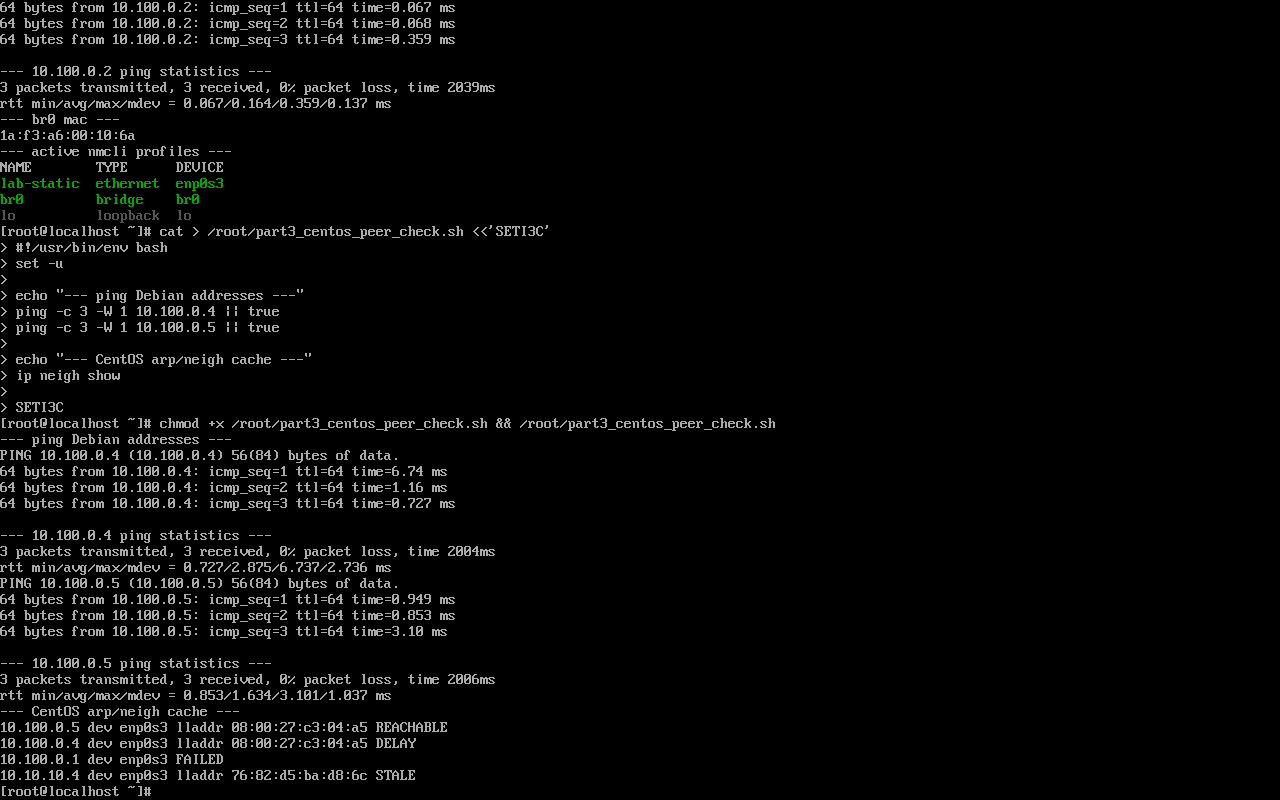
\includegraphics[width=\linewidth]{centos9-part3-peer.png}
\caption{CentOS: обратный ping Debian и ARP-кэш}
\end{figure}

\section{Часть 4. Bonding}

Для проверки bonding у Debian был добавлен второй сетевой адаптер. Оба адаптера временно переводились в режим \texttt{NAT Network} с сетью \texttt{lab-nat} и включенным DHCP. Внутри Debian был загружен модуль \texttt{bonding}, создан bonding-интерфейс \texttt{bond007} в режиме round-robin.

\lstinputlisting[caption={Скрипт настройки bonding}]{part4_bonding_runtime.sh}

Результат:
\begin{itemize}
  \item создан интерфейс \texttt{bond007};
  \item режим bonding: \texttt{load balancing (round-robin)};
  \item DHCP выдал адрес \texttt{10.10.10.4/24};
  \item маршрут по умолчанию установлен через \texttt{10.10.10.1};
  \item slave-интерфейсы: \texttt{enp0s3} и \texttt{enp0s8};
  \item MAC \texttt{enp0s3}: \texttt{08:00:27:c3:04:a5};
  \item MAC \texttt{enp0s8}: \texttt{08:00:27:b0:d3:f8}.
\end{itemize}

\begin{figure}[H]
\centering
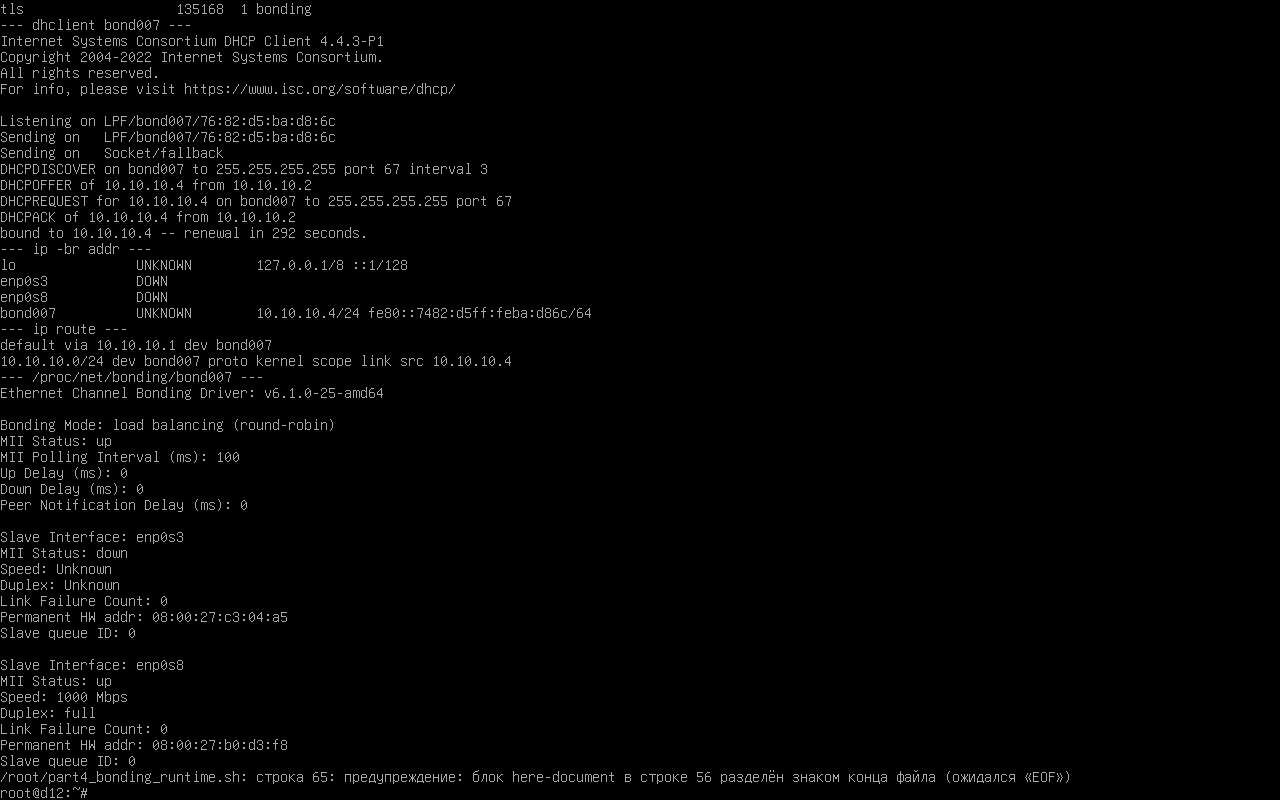
\includegraphics[width=\linewidth]{debian12-part4-output.png}
\caption{Debian: создание bond007 и вывод /proc/net/bonding/bond007}
\end{figure}

\subsection{Скрипт статистики}

Для анализа счетчиков был создан скрипт, который выводит текущее время, имя интерфейса, количество принятых и отправленных пакетов по данным \texttt{/proc/net/dev}.

\lstinputlisting[caption={Скрипт статистики интерфейса bond007}]{part4_iface_stats.sh}

Во время выполнения \texttt{ping -I bond007 -c 8 8.8.8.8} скрипт статистики был запущен три раза. Значения счетчиков увеличивались:
\begin{itemize}
  \item \texttt{18:49:41}: RX packets = 123, TX packets = 135;
  \item \texttt{18:49:43}: RX packets = 126, TX packets = 138;
  \item \texttt{18:49:45}: RX packets = 130, TX packets = 142.
\end{itemize}

Пакеты к \texttt{8.8.8.8} через VirtualBox NAT Network получили 100\% loss, но увеличение TX/RX-счетчиков показывает, что трафик через \texttt{bond007} формировался и обрабатывался интерфейсом. В выводе \texttt{/proc/net/dev} также видно распределение статистики между \texttt{enp0s3}, \texttt{enp0s8} и \texttt{bond007}.

\begin{figure}[H]
\centering
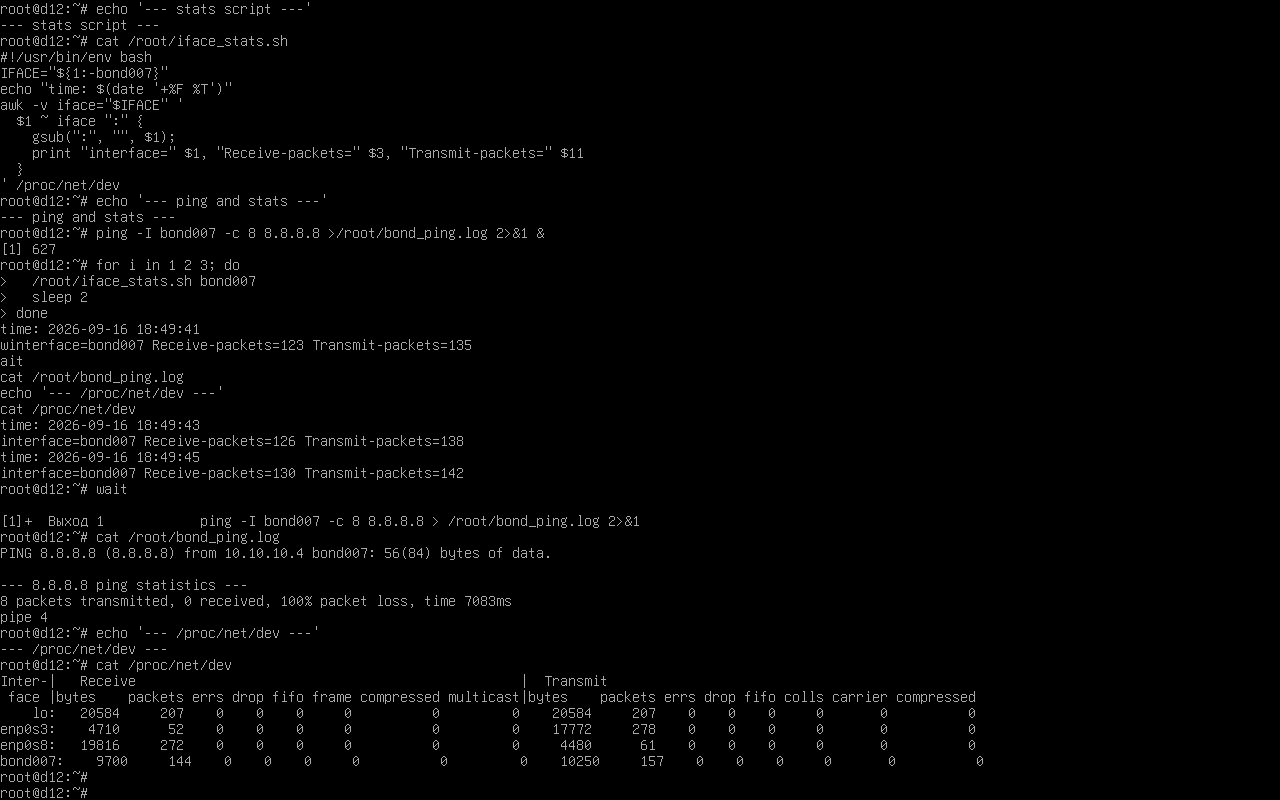
\includegraphics[width=\linewidth]{debian12-part4-stats.png}
\caption{Debian: статистика bond007 во время ping}
\end{figure}

\section{Ответы на контрольные вопросы}

\subsection{Команды ip}

\begin{itemize}
  \item Назначить IPv4-адрес: \texttt{ip addr add 10.100.0.2/24 dev enp0s3}.
  \item Изменить MAC-адрес: \texttt{ip link set dev enp0s3 address 02:11:22:33:44:55}.
  \item Назначить gateway: \texttt{ip route replace default via 10.100.0.1 dev enp0s3}.
  \item Показать ARP-кэш: \texttt{ip neigh}.
  \item Очистить ARP-кэш: \texttt{ip neigh flush all}.
  \item Включить интерфейс: \texttt{ip link set enp0s3 up}.
  \item Выключить интерфейс: \texttt{ip link set enp0s3 down}.
\end{itemize}

\subsection{Duplex}

Half duplex означает, что устройство в один момент времени либо передает, либо принимает данные. Full duplex позволяет одновременно передавать и принимать данные. Auto negotiation используется для автоматического согласования скорости и duplex между устройствами.

\subsection{Несколько IP-адресов на одном интерфейсе}

Несколько IP-адресов на одном интерфейсе применяются для размещения нескольких сервисов, миграции адресов, виртуального хостинга, отказоустойчивости, работы с несколькими подсетями и временной совместимости при перенумерации сети.

\subsection{Виртуальные интерфейсы}

Виртуальные интерфейсы используются для bridge, VLAN, контейнеров, маршрутизации, лабораторных стендов, изоляции трафика и тестирования сетевых сценариев без добавления физических сетевых карт.

\subsection{Режимы bonding}

\begin{itemize}
  \item \texttt{balance-rr} / mode 0: round-robin, поочередная передача пакетов через slave-интерфейсы.
  \item \texttt{active-backup} / mode 1: один активный интерфейс и резервный интерфейс для отказоустойчивости.
  \item \texttt{balance-xor} / mode 2: выбор интерфейса по хешу.
  \item \texttt{broadcast} / mode 3: отправка пакетов через все slave-интерфейсы.
  \item \texttt{802.3ad} / mode 4: LACP-агрегация, требует поддержки на коммутаторе.
  \item \texttt{balance-tlb} / mode 5: адаптивная балансировка исходящего трафика.
  \item \texttt{balance-alb} / mode 6: адаптивная балансировка исходящего и входящего трафика.
\end{itemize}

\section{Вывод}

В ходе работы были настроены сетевые интерфейсы Linux разными способами: runtime-командами \texttt{ip}, через \texttt{nmcli} на CentOS, через подготовленный YAML-файл \texttt{netplan} на Debian и через bonding-интерфейс \texttt{bond007}. Проверка связи между CentOS и Debian подтвердила работоспособность внутренней сети \texttt{seti-lab}. В bonding-сценарии был создан интерфейс round-robin, получен DHCP-адрес и проанализированы счетчики трафика в \texttt{/proc/net/dev}.

\end{document}
